\documentclass[11pt,a4paper]{article}
\usepackage[utf8]{inputenc}
\usepackage[T1]{fontenc}
\usepackage{amsmath}
\usepackage{amsfonts}
\usepackage{amssymb}
\usepackage[left=3.0cm, right=3.0cm, top=3.0cm, bottom=3.0cm]{geometry}
\usepackage{xcolor}
\usepackage{graphicx}
\usepackage{caption}
\usepackage{subcaption}

% include code listings
\usepackage{listings}

% Defining colors for syntax highlighting
\definecolor{codegreen}{rgb}{0,0.6,0}
\definecolor{codegray}{rgb}{0.5,0.5,0.5}
\definecolor{codepurple}{rgb}{0.58,0,0.82}
\definecolor{backcolour}{rgb}{0.95,0.95,0.92}

\lstdefinestyle{mystyle}{
	backgroundcolor=\color{backcolour},   
	commentstyle=\color{codegreen},
	keywordstyle=\color{magenta},
	numberstyle=\tiny\color{codegray},
	stringstyle=\color{codepurple},
	basicstyle=\ttfamily\scriptsize,
	breakatwhitespace=false,         
	breaklines=true,                 
	captionpos=b,                    
	keepspaces=true,                 
	numbers=left,                    
	numbersep=5pt,                  
	showspaces=false,                
	showstringspaces=false,
	showtabs=false,                  
	tabsize=2
}

\lstset{style=mystyle}
\captionsetup[lstlisting]{font={scriptsize}}

% header and footer
\usepackage{fancyhdr}
\pagestyle{fancy}
\fancyhf{}
\lhead{Michele Guadagnini}
\rhead{\today}
\lfoot{Street features detection - Computer Vision 2021}
\rfoot{Page \thepage}

\author{Michele Guadagnini - ID 1230663}
\title{\textbf{Computer Vision 2021 - Homework (LAB 3): \\ \textit{Street features detection}}}
\date{\today}


\begin{document}
\maketitle

\vspace{20pt}
\begin{abstract}
	The goal of this homework is to detect and highlight the \textbf{street lanes} and the \textbf{round street signs} from some pictures. The program exploits the \textit{Canny} edge detection algorithm and the \textit{Hough} transform to complete the task. The detected features will be highlighted by coloring the corresponding pixels. \\
	The code has been developed in \textit{C++} language, making use of the \textit{OpenCV} library. Almost all the parameters of the applied algorithms can be set making use of trackbars; this allows to easily select the best parameters.
\end{abstract}

\section{Implementation description} %Explain briefly the theory you have based your solution on.

The solution of the task has been developed by creating a library containing the functions to be called in the main program. The most important ones are:

\begin{itemize}
	\item \textit{DetectEdges}: it uses the Canny algorithm to detect the edges to be passed to the Hough transform. The function convert the input image to gray-scale and creates the two trackbars needed to tune the two threshold of the algorithm.
	
	\item \textit{RetrieveLines}: it applies the Hough transform to the edges computed above in order to detect the street lanes. It creates 5 trackbars for the parameters. When using it, the parameters has been tuned to detected the right-most street lane, although it was not always possible.
	
	\item \textit{RetrieveCircles}: it is used to detect the round signs in the images. Before passing the image to the \textit{OpenCV} function \textbf{cv::HoughCircles}, a gaussian filter is applied in order to reduce the noise; the \textit{sigma} of the filter must be passed as a parameter to the command line. Then, the function converts the image to gray-scale and creates the trackbars.
	
	\item \textit{SaveResult}: it overlaps the detected regions with the colors defined at the top of the library implementation file \textit{street\_features\_utils.cpp}: circles will be filled with green, lines are drawn with red and the region between lines with purple.
\end{itemize} 

The library contains some other functions used to apply the gaussian filter and to compute the points representing the polygon of the region between detected lines. \\
Also a callback function for each of the first three functions above have defined, that are used when the parameters values are changed using the corresponding trackbar. To pass the image and some parameters to the callbacks, a simple class has been defined (see \textit{street\_features\_utils.h}). \\

The program requires 4 arguments to be passed on command line: 
\begin{itemize}
	\item the name of the input image file;
	\item the name of the output file;
	\item a string that contains the type of desired output. The possible options are "\textit{region}", which overlaps a colored polygon to the region between the detected lines; "\textit{lines}", which draws only the lines; "\textit{both}", which plots both lines and region.
	\item the $\sigma$ of the gaussian filter to be applied before circles detection. If $\sigma < 2$, filtering is skipped. 
\end{itemize}
In case of wrong number of arguments, the program prints a help message with instructions.

\subsection{Compilation and usage}

The program has been compiled with the following command:
\begin{lstlisting}[language=BASH,numbers=none]
	g++ -o street_features street_features_main.cpp street_features_utils.cpp `pkg-config --cflags --libs opencv`
\end{lstlisting}

Below it is reported a usage explanation of the executable:
\begin{lstlisting}[language=BASH,numbers=none] 
	./street_features [input_name] [output_name] [plot_option] [gaussian_sigma]
\end{lstlisting}


\section{Results} %Present data and explain your results.

The provided images has been analyzed with the program. The optimal parameters used in the analysis are reported in Table \ref{tab:edges}, Table \ref{tab:lines} and Table \ref{tab:circles}.

% tabelle con i parametri usati
\begin{table}[b]
	\begin{center}
		\begin{tabular}{ccc}
			\hline
			 \multicolumn{3}{c}{\textbf{Canny edge detection}}   \\
			\textit{image} & low threshold & high threshold \\ \hline
			  road1    &      436      &      917       \\
			  road2    &      495      &      862       \\
			  road3    &      192      &      302       \\
			  road4    &      490      &      730       \\
			  road5    &      628      &      885       \\
			  road6    &      530      &      768       \\
			  road7    &      148      &      355       \\
			  road8    &      271      &      816       \\ \hline
		\end{tabular}
	\end{center}
	\caption{}
	\label{tab:edges}
\end{table} 
\begin{table}
	\begin{center}
		\begin{tabular}{cccccc}
			\hline
			    \multicolumn{6}{c}{\textbf{Hough transform lines detection}}      \\
			\textit{image} & $\rho$ res. & $\theta$ res. & Counts & min $\theta$ & max $\theta$ \\ \hline
			  road1    &    1    &     2      &    170    &     2     &    115    \\
			  road2    &    1    &     1      &    105    &     0     &    180    \\
			  road3    &    1    &     2      &    280    &     0     &    180    \\
			  road4    &    1    &     2      &    129    &     0     &    180    \\
			  road5    &    2    &     2      &    92     &    109    &    123    \\
			  road6    &    2    &     2      &    47     &    136    &    180    \\
			  road7    &    1    &     2      &    83     &     0     &    180    \\
			  road8    &    1    &     2      &    98     &     0     &    180    \\ \hline
		\end{tabular}
	\end{center}
	\caption{}
	\label{tab:lines}
\end{table} 
\begin{table}
	\begin{center}
		\begin{tabular}{ccccccc}
			\hline
			              \multicolumn{7}{c}{\textbf{Hough transform circles detection}}               \\
			\textit{image} & min distance & canny high & Counts & min radius & max radius & gaus. $\sigma$ \\ \hline
			  road2    &      10      &    100     &   23   &     1      &    500     &       4        \\
			  road3    &     200      &     96     &   24   &     1      &     77     &       3        \\
			  road4    &      5       &    115     &   16   &     1      &    500     &       4        \\
			  road7    &      20      &     70     &   15   &     1      &    500     &       4        \\
			  road8    &      20      &     32     &  100   &     1      &    280     &       4        \\ \hline
		\end{tabular}
	\end{center}
	\caption{}
	\label{tab:circles}
\end{table} 

Below instead are reported some comparisons between original and successfully processed images (Figure \ref{fig:img1} and Figure \ref{fig:img2}). The target for the lines detection was the right-most street lane, although sometimes filter out the spurious lines has not been possible without additional conditions with respect to the parameters on trackbars (see Figure \ref{fig:bad}).

Other results are included the \textit{.zip} archive.

% immagini con confronto (2 o 3 coppie al massimo)
\begin{figure}[h]
	\centering
	\begin{subfigure}{1\textwidth}
		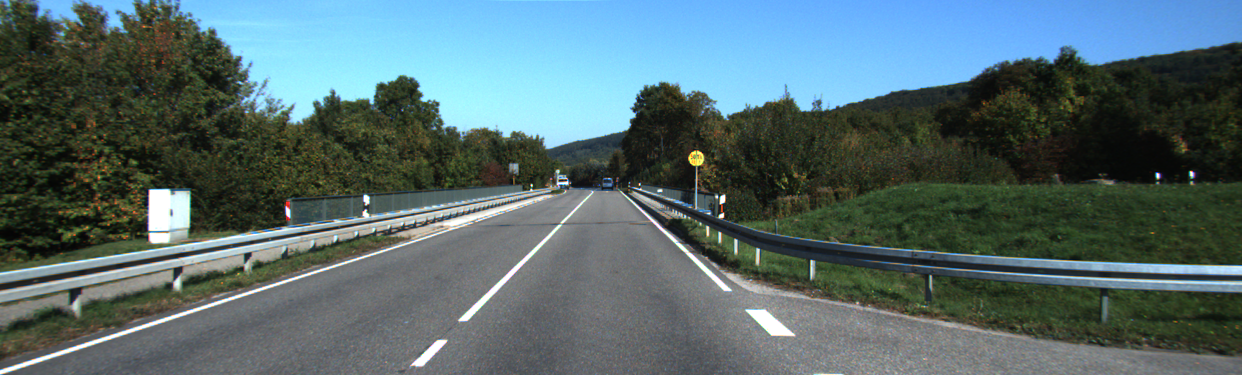
\includegraphics[width=1\linewidth]{road2.png}
	\end{subfigure}%
    \hfill
    \vspace{10pt}
	\begin{subfigure}{1\textwidth}
		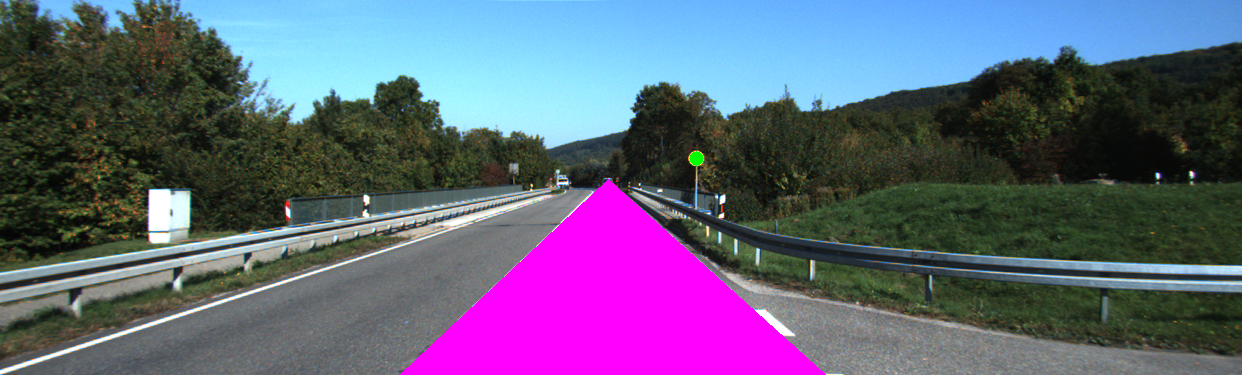
\includegraphics[width=1\linewidth]{road2_featured.png}
	\end{subfigure}
	\hfill
	\vspace{10pt}
	\caption{ }
	\label{fig:img1}
\end{figure}

\begin{figure}[h]
	\centering
	\begin{subfigure}{0.49\textwidth}
		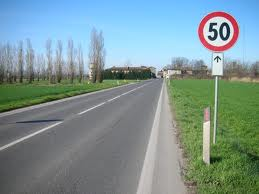
\includegraphics[width=1\linewidth]{road7.jpg}
	\end{subfigure}%
	\hfill
	\begin{subfigure}{0.49\textwidth}
		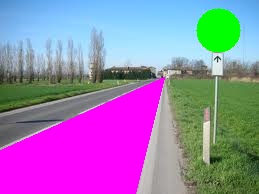
\includegraphics[width=1\linewidth]{road7_featured.jpg}
	\end{subfigure}
	\caption{ }
	\label{fig:img2}
\end{figure}

\begin{figure}[h]
	\begin{subfigure}{1\textwidth}
		\centering
		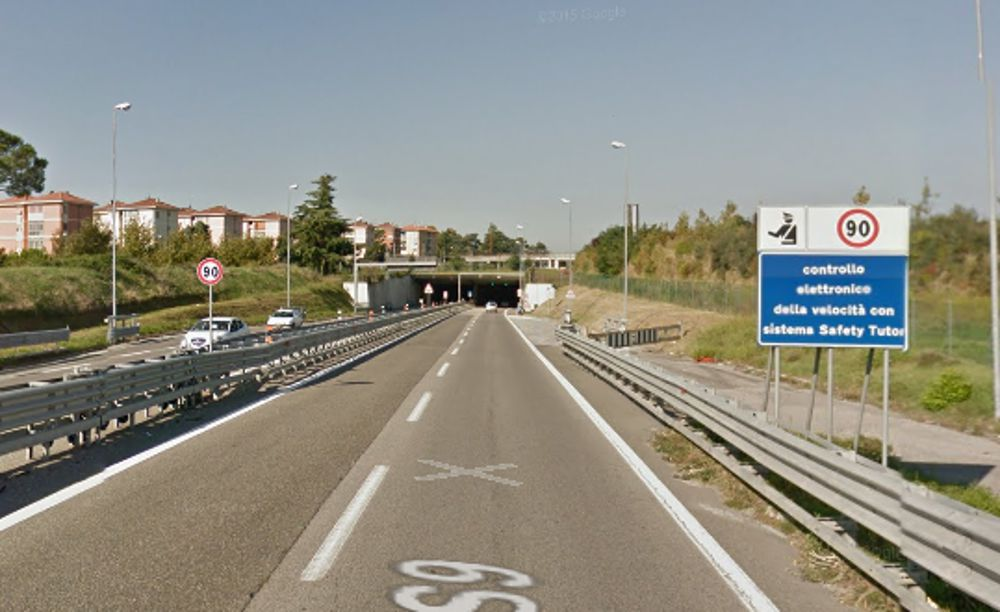
\includegraphics[width=0.7\linewidth]{road3.jpg}
	\end{subfigure}%
	\hfill
	\vspace{10pt}
	\begin{subfigure}{1\textwidth}
		\centering
		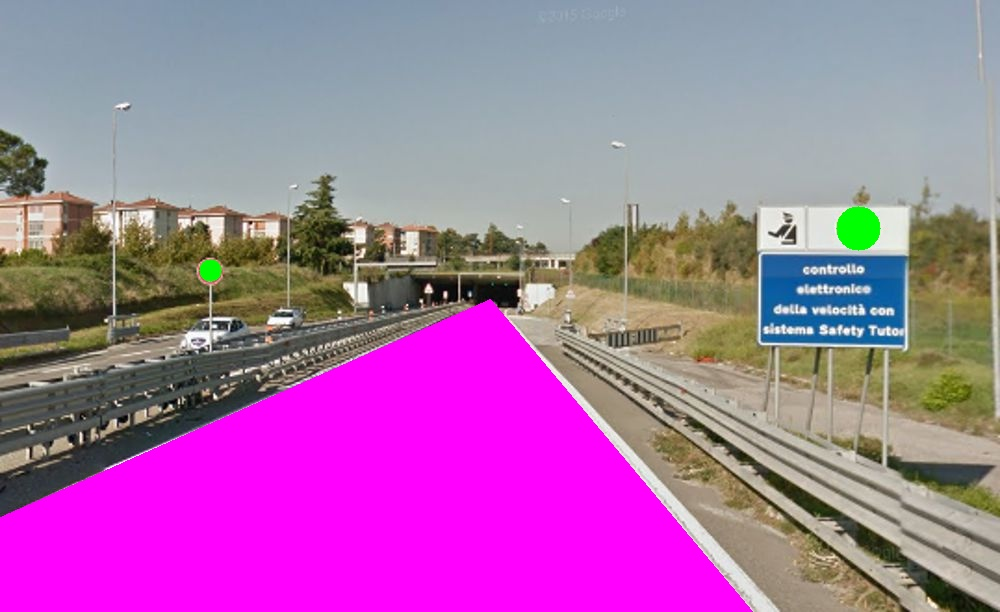
\includegraphics[width=0.7\linewidth]{road3_featured.jpg}
	\end{subfigure}
	\hfill
	\vspace{10pt}
	\caption{ }
	\label{fig:bad}
\end{figure}



%\begin{figure}[h]
%	\centering
%	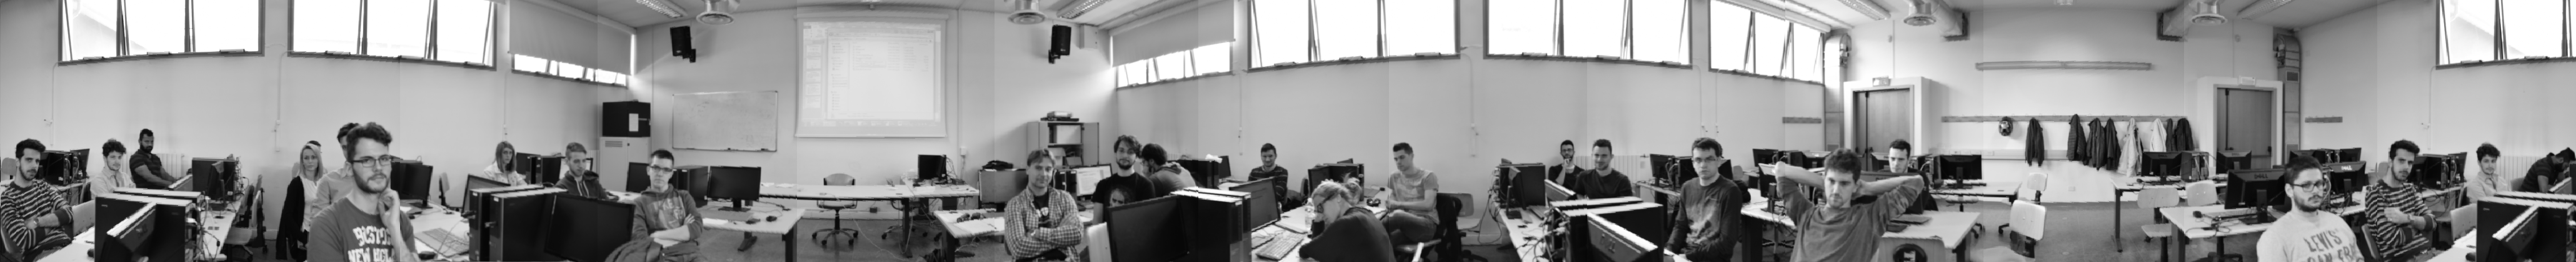
\includegraphics[width=1\linewidth]{lab_pan_gray.png}
%	\caption{Laboratory panoramic view in gray-scale.}
%	\label{fig:lab_g}
%\end{figure}


\end{document}
